\section*{Appendix A: Project Budget}
\addcontentsline{toc}{section}{Appendix A: Project Budget}
The project has been completed with a total budget of NPR 41,160. This budget covers various aspects of the project, including computation resources, cloud services, IEEE membership, and miscellaneous expenses.

\begin{table}[H]
    \centering
    \small
    \caption{Project Budget Breakdown}
    \begin{tabular}{p{3.5cm}p{5.5cm}c}
        \toprule
        \textbf{Category} & \textbf{Details} & \textbf{Estimated Cost (NPR)} \\
        \midrule
        Computation Requirements & Google Colab Pro (\$9.99 per month), NVIDIA T4 GPU (\$0.35 per hour), Lightning AI Credits & 24,000 \\
        IEEE Xplore Membership & Annual subscription for accessing research articles, journals & 2,160 \\
        Miscellaneous Costs & Report printing, binding, API, etc. & 15,000 \\
        \midrule
        Total & & \textbf{41,160} \\
        \bottomrule
    \end{tabular}
    \label{tab:project_budget}
\end{table}

\clearpage
\section*{Appendix B: Gantt Chart}
\addcontentsline{toc}{section}{Appendix B: Gantt Chart}

\begin{table}[htbp]
\centering
\resizebox{\textwidth}{!}{%
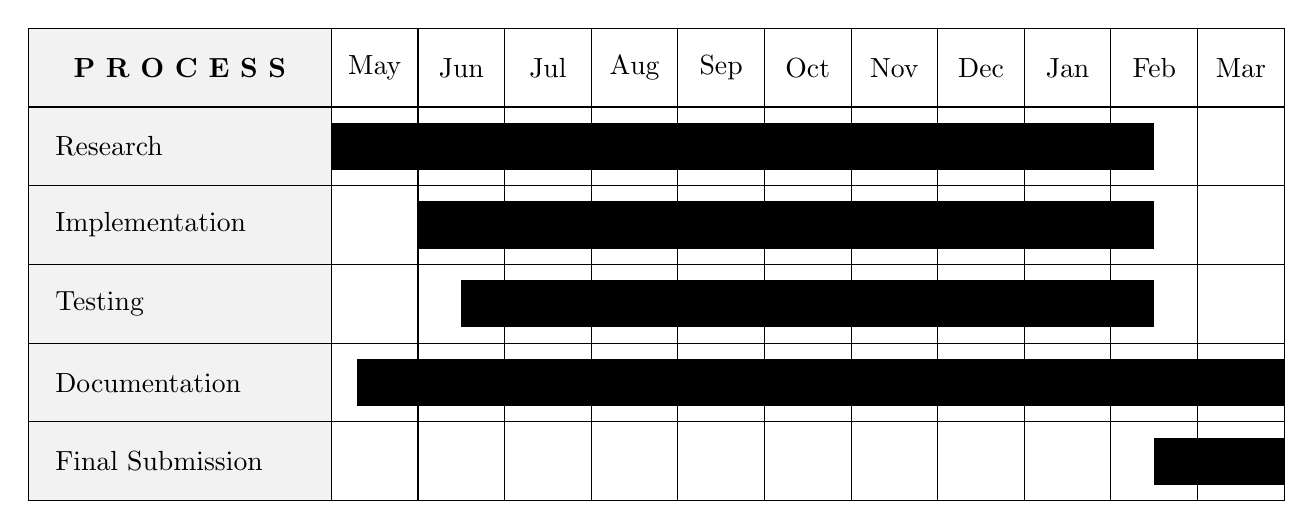
\begin{tikzpicture}[x=1.1cm, y=1cm]
    % --- Configuration ---
    \def\colW{3.5}    % Width of the PROCESS column
    \def\monthW{1}    % Width of each month column
    \def\rowH{-1}     % Height of each row (negative for downward growth)
    \def\numMonths{11}
    \def\numRows{6}

    % --- Background for PROCESS column ---
    \fill[gray!10] (0, 0) rectangle (\colW, 6 * \rowH);

    % --- Grid Lines ---
    % Horizontal lines
    \foreach \i in {0,...,6} {
        \draw[thin] (0, \i * \rowH) -- ({\colW + \numMonths * \monthW}, \i * \rowH);
    }
    
    % Vertical lines
    \draw[thin] (0, 0) -- (0, 6 * \rowH); % Far left
    \draw[thin] (\colW, 0) -- (\colW, 6 * \rowH); % Process column boundary
    
    % Month boundaries (skipping the line in the middle of February)
    \foreach \j in {1,...,11} {
        \draw[thin] ({\colW + \j * \monthW}, 0) -- ({\colW + \j * \monthW}, 6 * \rowH);
    }

    % --- Headers ---
    \node[anchor=center, font=\bfseries] at ({\colW/2}, 0.5 * \rowH) {P R O C E S S};
    
    \foreach \m [count=\i] in {May, Jun, Jul, Aug, Sep, Oct, Nov, Dec, Jan, Feb, Mar} {
        \node[anchor=center] at ({\colW + (\i - 0.5) * \monthW}, 0.5 * \rowH) {\m};
    }

    % --- Task Labels ---
    \foreach \label [count=\i] in {Research, Implementation, Testing, Documentation, Final Submission} {
        \node[anchor=west] at (0.2, {\i * \rowH + 0.5 * \rowH}) {\label};
    }

    % --- Gantt Bars ---
    % Pre-calculating values for clean coordinates
    \def\barHeight{0.6}
    \pgfmathsetmacro{\topPadding}{(1-\barHeight)/2}
    \pgfmathsetmacro{\bottomPadding}{\topPadding + \barHeight}

    % Task 1: Research (May to Mid-Feb)
    \fill[black] (\colW, {1 * \rowH + \topPadding * \rowH}) rectangle ({\colW + 9.5 * \monthW}, {1 * \rowH + \bottomPadding * \rowH});

    % Task 2: Implementation (Jun to Mid-Feb)
    \fill[black] ({\colW + 1 * \monthW}, {2 * \rowH + \topPadding * \rowH}) rectangle ({\colW + 9.5 * \monthW}, {2 * \rowH + \bottomPadding * \rowH});

    % Task 3: Testing (Jul to Mid-Feb)
    \fill[black] ({\colW + 1.5 * \monthW}, {3 * \rowH + \topPadding * \rowH}) rectangle ({\colW + 9.5 * \monthW}, {3 * \rowH + \bottomPadding * \rowH});

    % Task 4: Documentation (May to End-Mar)
    \fill[black] ({\colW + 0.3 * \monthW}, {4 * \rowH + \topPadding * \rowH}) rectangle ({\colW + 11 * \monthW}, {4 * \rowH + \bottomPadding * \rowH});

    % Task 5: Final Submission (Mid-Feb to End-Mar)
    \fill[black] ({\colW + 9.5 * \monthW}, {5 * \rowH + \topPadding * \rowH}) rectangle ({\colW + 11 * \monthW}, {5 * \rowH + \bottomPadding * \rowH});

\end{tikzpicture}%
}
\caption{Project Timeline (Gantt Chart)}
\label{tab:gantt}
\end{table}
